\documentclass[12pt]{article}

\usepackage{amssymb,amsmath,amsfonts,eurosym,geometry,ulem,graphicx,caption,color,setspace,sectsty,comment,footmisc,caption,natbib,pdflscape,subfigure,array,hyperref}

\normalem

\onehalfspacing
\newtheorem{theorem}{Theorem}
\newtheorem{corollary}[theorem]{Corollary}
\newtheorem{proposition}{Proposition}
\newenvironment{proof}[1][Proof]{\noindent\textbf{#1.} }{\ \rule{0.5em}{0.5em}}

\newtheorem{hyp}{Hypothesis}
\newtheorem{subhyp}{Hypothesis}[hyp]
\renewcommand{\thesubhyp}{\thehyp\alph{subhyp}}

\newcommand{\red}[1]{{\color{red} #1}}
\newcommand{\blue}[1]{{\color{blue} #1}}

\newcolumntype{L}[1]{>{\raggedright\let\newline\\arraybackslash\hspace{0pt}}m{#1}}
\newcolumntype{C}[1]{>{\centering\let\newline\\arraybackslash\hspace{0pt}}m{#1}}
\newcolumntype{R}[1]{>{\raggedleft\let\newline\\arraybackslash\hspace{0pt}}m{#1}}

\geometry{left=1.0in,right=1.0in,top=1.0in,bottom=1.0in}

\begin{document}

\section{Introduction}

We examine collective memories of the European debt crisis that
began in 2010: memories of experts and non-experts, considering whether they are from program countries or non-program countries.
The European debt crisis partitioned the countries inside the Eurozone. Some
Eurozone member countries experienced fiscal and financial conditions that
dramatically worsened and were in danger of losing access to the capital
market for refinancing their public loans. The other countries had to
fear contagion effects and spillovers of possible national
bankruptcies in the more severely affected countries.\ Five countries
(Greece, Ireland, Portugal, Spain and Cyprus) applied for, and signed a
memorandum of understanding with the member countries of the European
Monetary Union. They received financial aid or
guarantees and accepted supervised mandatory structural reforms. We refer to the program
countries as the 'borrower countries'. Other countries used their fiscal credibility to provide these guaranties and requested
and participated in a monitoring of the process of structural reforms. We
refer to them as 'lender countries'.

Will citizens from borrower and lender countries have similar memories about who
applied for a memorandum of understanding? How do they remember
whether the lender or the borrower countries pushed for the memoranda of understanding and whether
the memoranda of understanding mainly benefited the lender countries or the
borrower countries? And if there are differences between borrower and lender countries, do these differ between economic experts and non-experts? We also
investigate how the programs were perceived in the countries
and how the crisis interventions influenced the relationship between
countries.\ 

We consider the views of experts polled by CESifo's World Economic Survey (WES) panel of experts and non-experts in European countries in an internet questionnaire (https://prolific.co) to answer the same questions. The results do not suggest that the answers between experts from borrower countries and experts from lender countries diverge. However, differences emerge in how non-experts from the borrower and lender countries remember which countries signed a memorandum, why they signed it, and how they assess the measures taken to address the crisis. We employ data from 2018/2019 (experts/non-experts) and examine whether the borrower or lender position predicts how the crisis is remembered and assessed. 

Memory formation has been primarily studied in psychology, neuroscience and sociology.
Insights about the plasticity of memory\footnote{%
The physiological basics for how memory is formed, kept and reactivated have
been explored. As Dudai and Edelson (2016;\ 276)\ describe, "When the memory
is retrieved, it seems to re-enter a transient phase in which it again
becomes susceptible to the same amnesic agents that were effective in the
original consolidation window (\cite{dudai}; \cite{nader}; Sara,
2000)." Brain sciences hence suggest that memory enters a state of
plasticity when it is reactivated and the copy that is then stored might
differ from the one that has been activated (see \cite{agren}, and \cite{lee}).}, and a tendency to memorize in a 'self-serving' way
(\cite{bell}) have been combined. If this self-serving bias
affects the process of reactivating, transforming and storing memory, it may well
cause memory with a self-serving bias.

A self-serving bias has been shown in memories of informal credit relationships (\cite{dezso}). Using data about informal credit
relationships between relatives and friends, \cite{dezso} find that borrowers and
lenders diverge in their memories about these credit relationships in self-serving
 ways.
Borrowers and lenders remember in different manners the credit event
as such, the conditions of the loan they agreed upon, and the mutual
interactions that made the contract come about. This divergence typically
has a self-serving bias. For instance, compared to the lenders, borrowers
tend to recall less if they exerted moral pressure to receive the loan and
are more likely to recall that the credit was generously offered to them.

The lenders and borrowers in the European debt crisis are
nations, no individuals, but the line of reasoning may well be
similar: when investigating the recollections of fiscal credit relationships or
loan guarantees between nations, the mental processes of the formation,
storage and reactivation of memory are still those of individuals.
The formation of memories of individuals who belong to the same group might
follow the same logic and physiological laws as in private
borrowing-lending relationships. Overall, individuals in borrower
countries and individuals in lender countries might recall differently
aspects of the credit relationship similar to individuals in a private credit relationship. 

\\

Diverging views and memories might be reinforced 
by biased public news and newspaper reports. Common
institutions inside a nation, such as common exposure to the same public
media and other public institutions might intensify information exchange
inside the group, might cause a continuous transformation of this aggregate
and might even strengthen and homogenize the national collections of
memories. For discussions see \cite{rigney} and Roediger and Abel (2015;\
361) who conclude: "Such collective memories probably boost group identity
and shape social and political discourse. In particular, studies of how
various groups remember `the same' events so differently may help to uncover
important psychological factors in group dynamics and conflict." \cite{baumeister} describe that groups employ techniques such as selective omission, fabrication of alternative narratives and exaggeration or embellishments of events to let their group appear in a favorable light. \cite{abel} show self-serving group bias in country's assessment of the Second World War. Citizens overestimate their country's contribution to the Second World War. 

We relate to studies which investigate how views of economic experts and non-experts differ. \cite{johnston} find that citizens are influenced by the views of economic experts, more so if the issue at stake is highly technical and less ideological. However, the issue at stake does not appear to be the only determinant of divergence in the views of experts and non-experts. In a survey of economic experts and a representative sample of the U.S. population \cite{sapienza} find that NIKLAS: WAS BEDEUTET DER KOMMENDE HALBSATZ? the divergences in opinions is increasing in the level of agreement among economic experts. The WES has also been employed to measure discrepancies in the views of experts and non-experts. \cite{roth} find that experts and non-experts assess the impact of macroeconomic shocks differently.

Our study is also related to studies in political science.
%We conduct an inter-country comparison  of memories of the events surrounding the European debt crisis and compare the memories of economic experts to regular citizens. 
\cite{bechtel} examine how the political orientation of German citizens influences attitudes towards the European debt crisis. The results show that traditional left/right cleavages do not explain participants perception of the European debt crisis but rather moderateness of political views. More cosmopolitan survey participants are less opposed to the European rescue program. This finding is corroborated by \cite{kuhn} who use survey data: ``cosmopolitans" have a lower propensity to discriminate between national recipients of transfers and international recipients of transfers than non-cosmopolitans. We designed a survey specific to the European debt crisis and ask experts and non-experts in European Union member states. We compare the memories of economic experts and non-experts. Examining a nation-serving bias in memorizing the European debt crisis is new. 



\section{The Design}
\subsection{The Sample}
Our data was obtained through a survey we conducted among two pools of participants. In August 2018, we asked economic experts from the World Economic Survey (WES) for their opinion on perceptions about the financial entrenchment following the European debt crisis. The WES is a quarterly survey conducted by the ifo Institute. The survey includes many  questions, indicating the opinion towards overall economic development from European and non-European  experts such as economic growth and inflation. The WES also includes special questions on current economic issues. Our WES sample includes 517 participants from EU member countries, among them 90 from program countries.
\\
Our second pool of participants was recruited through the website prolific.co.In contrast to other crowdsourcing platforms such as Mturk Prolific is a platform specifically designed to recruit participants for academic research \footnote{\cite{Peer} demonstrate that participants from the platform prolific perform better than participants from other crowdsourcing platforms}. In exchange for their participation in surveys or experiments, participants receive a financial reward. The survey was distributed to 1702 participants in August 2019, 498 of these participants came from program countries. To ensure that our participants actively remember the events during the European debt crisis we restrict our sample to include only participants older than 25. \\
Participants from both samples received the survey questions in the same ordering. The appendix shows the origin of survey participants from both samples.  
\subsection{Sample Characteristics} 
The WES sample and the prolific sample differ along various dimensions. More than 80 percent of WES participants are male, whereas in the prolific sample there is an equal share of men and women. The majority of participants from the prolific sample, around 65 percent are younger than 35, whereas the majority of participants from the WES sample are between 35 and 55. Participants from the WES sample are also have a higher level of education than participants from the prolific sample, 60 percent of participants hold a PhD. Nonetheless the majority of participants from the prolific sample have completed tertiary education. We henceforth refer to the WES sample as the expert sample and to the prolific sample as the non-expert sample. 
\subsection{Survey Structure}
Our survey contains seven main questions about participants recollection of various aspects of the European debt crisis consisting of several  We base our questions on the survey conducted by \cite{dezso}. We use two types of questions to examine whether citizens from borrower countries perceive the European debt crisis in a different manner than citizens from from lender countries. First, we ask experts to assess their level of agreement with a certain statement on a scale of 1 to 4. Second we ask participants to name a party to which a certain statement applies. Participants can name the borrower countries, the lender countries our both equally. We further ask participants which countries participated in the European debt crisis and collect information on socioeconomic characteristics. We ask participants from the prolific sample and the WES sample to indicate their level of education, age, gender. Participants from the prolific sample are also asked to name their employment status, WES participants to name their affiliation. 

\section{The  Hypotheses}
We expect our participants to show a nation-serving bias in their answers to our survey questions. In the following we predict how the answers of participants from program countries will differ with regard to the answers of participants from non-program countries. The full set of survey questions is shown in the appendix. 


\begin{enumerate} 
\item\textbf{Why the lender countries engaged in the credit relationship} \\
We ask participants whether lender countries acted out of benevolence (to help the borrower countries) or out of self-interest (to avoid a crisis in their own countries/to force institutional change upon the borrower countries). We predict that participants from program countries are more likely to state that lender countries acted out of self-interest and less likely that they acted out of benevolence. 

\item \textbf{Who initiated the credit relationship} \\
We ask our survey participants to assess which party was the driving force behind the credit relationship. We predict that participants from program countries will be more likely to state that citizens from lender countries initiated the credit relationship. 

\item \textbf{Which party benefited from the rescue program}\\ 
We first ask participants whether borrower or lender countries were the main beneficiaries of the rescue program. In a subsequent question we also ask whether Greece was the main beneficiary from the rescue program. For both answers we expect that participants from program countries will be more likely to state that lender countries were the main beneficiaries from the rescue program. 

\item \textbf{ What feelings the rescue program evoked among citizens from program and non-program countries}\\
Our participants are asked whether the rescue program evoked negative feelings among citizens from borrower countries (feeling guilty, exploited or inferior). Further, they are asked whether the rescue program evoked negative feelings among the lender countries (feelings of exploitation and disappointment).  
We expect participants from program countries to be more likely to agree that the rescue program evoked negative feelings among citizens from borrower countries and less likely to state that the rescue program evoked negative feelings among citizens from non-program countries. 
\item \textbf{Whether outstanding debt will be repaid} \\
We ask participants if Greece will be able to repay it's outstanding debt. \footnote{Greece is the only country which has not repaid the loans it received in the course of the rescue program} We expect citizens from program countries to demonstrate more confidence in Greece's ability to repay outstanding debt. 
\end{enumerate}

\section{Descriptive Statistics}

\textbf{Comparison of Means}
We compare the mean answers of the experts with the mean answers of non-experts from program and non-program countries to determine whether experts side more with the opinion of borrower or lender countries.\\
When asked about the intentions of the lender countries experts do not show a tendency to side with neither non-experts from program countries or non-experts from non-program countries. They are slightly more likely to agree that lender countries wanted to help borrower countries than non-experts, more along the lines of non-experts from non-program countries. Further, they are more likely to agree that lender countries engaged in the rescue program out of self-interest siding with the borrower countries on this issue. The lack of agreeing with either side also emerges when expert are asked about the emotions the rescue program evoked among citizens from borrower and lender countries respectively. Overall, experts agree with the statements that citizens in borrower countries felt exploited and inferior more than non-experts. Hence, on this issue the opinion of experts resembles the opinion of non-experts from program countries. However, they also agree more to the statement that citizens in lender countries felt disappointed than non-experts. Experts from program and non-program countries only show statistically significant different level of agreements with the statement that Greece will fully pay back it's debt. For this question the average level of agreement in the expert and non-expert sample are similar for participants from program and non-program countries. \\
One interesting result emerges when experts are asked to assess to which party a certain statement applies. The answers from experts show some divergence on this matter, but in an opposite direction than non-experts. Experts from non-program countries are more likely to agree that their countries, the lender countries, were the main beneficiaries of the rescue program and loans to Greece. Further, experts from non-program countries are also more likely to agree than experts from program countries that lender countries were the driving force behind signing the referendum. However, it is important to note that these differences are not significantly different from zero.  \\

\textbf{Comparison of program countries} 
We compare the responses from participants of different program countries of the non-expert sample. We find that even within program countries survey participants in our non-expert sample diverge in their assessment of the European debt crisis. When asked about the intentions behind the rescue program it appears that Greek citizens show the strongest difference with respect to participants from non-program countries. Compared with the average assessment of program countries Greek participants are 20 percentage points less likely to agree that the lender countries wanted to help the borrowing countries, but strongly agree that the lender countries wanted to avoid a crisis at home and impose institutional change upon the borrower countries. In comparison to Greek participants other participants answer in a more moderate way. Notably, participants from Ireland are even 19 percentage points less likely to agree that lender countries wanted to impose institutional change than the average of program countries. The deviation of Greek participants is reinforced throughout the remaining survey questions. Participants from Greece agreed more strongly than participants from other program countries that the rescue program evoked feelings of guilt, exploitation and inferiority among citizens from the borrower countries (Question 5.1, 5.2, 5.3). Further, they are 14 and 16 percentage points less likely than citizens from program and non-program countries to agree that the rescue program strengthened friendships (Question(5.6). Contrary to our hypotheses Greek participants are also more likely to agree that the rescue program evoked negative feelings among the lender countries as well compared to the average of program countries (Question 5.4, 5.5).  They are more likely to agree that Greece will be able to pay it's debt, however the effect is not very large (Question 6). Greek participants strongly agree that the lender countries were the main beneficiaries of the loans to program countries and Greece and were also the main driving force behind initiating the rescue program (Questions 3, 4, 7).  All other program countries, which have already succeeded in repaying their debt show a weaker self-serving bias than Greek citizens. 
\\
Due to the small size of our expert sample we refrain from running inter-country comparisons. 


 \begin{table}[h!]
\caption{ Comparison of Means between individual program country and sample means} 
\resizebox{\textwidth}{!}{%
\begin{tabular}{*{7}{>{\centering\arraybackslash}p{.13\linewidth}}}
\hline\hline
&\multicolumn{4}{c}{\textbf{Deviation from the Program Country Mean}} &\multicolumn{2}{c}{\textbf{Means}} \\
           Question &\multicolumn{1}{c}{Greece}&\multicolumn{1}{c}{Ireland}&\multicolumn{1}{c}{Portugal}&\multicolumn{1}{c}{Spain}&\multicolumn{1}{c}{Program (mean)}&\multicolumn{1}{c}{Non-Program (mean) }\\
  
\hline
2.1 (-)       &       -0.20&        0.11&       -0.04&        0.03&        0.51&        0.62\\
2.2 (+)        &        0.05&        0.01&       -0.03&       -0.06&        0.91&        0.90\\
2.3 (+)       &        0.13&       -0.19&        0.03&       -0.08&        0.74&        0.62\\
\hline
&&&&&& \\
5.1 (+)        &        0.11&        0.04&       -0.05&       -0.02&        0.47&        0.39\\
5.2 (+)        &        0.14&       -0.05&       -0.01&       -0.16&        0.79&        0.61\\
5.3 (+)        &        0.10&        0.03&       -0.10&       -0.04&        0.72&        0.62\\
5.4 (-)        &        0.13&       -0.10&       -0.03&       -0.04&        0.60&        0.60\\
5.5 (-)        &        0.08&       -0.18&       -0.03&       -0.04&        0.61&        0.61\\
5.6  ()       &       -0.14&        0.10&        0.05&        0.02&        0.25&        0.27\\
\hline
&&&&&& \\
6  (+)         &        0.04&       -0.02&       -0.02&        0.03&        0.32&        0.18\\
3  (+)          &        0.14&        0.03&       -0.12&       -0.03&        0.54&        0.43\\
4  (+)          &        0.17&        0.03&        0.05&       -0.17&        0.67&        0.44\\
7  (+)          &        0.31&       -0.11&       -0.06&       -0.12&        0.55&        0.36\\
\hline\hline

\end{tabular} }
\begin{tablenotes}
\footnotesize
\item The sign in parantheses denotes the expectation about the difference in assessments between program and non-program countries. The left-hand side illustrates the difference between single program countries and the overall program country mean. The right hand side shows the program country mean and the non-program country mean. 
\end{tablenotes}
\end{table}


\clearpage
\section{Results}
We present the results of our empirical analysis for the sample of experts (the WES sample) and the sample of non-experts (the prolific sample).  We estimate the following model using binary logit. 
\begin{equation*}
    Y_{ijc}= \alpha_{j}+ \beta *D_{c} + \gamma*X_{i}
\end{equation*}
Where $Y_{ijc}$ denotes the response of individual $i$ from country $c$ to question $j$ we will control for individual characteristics $X_{i}$ such as age, level of education, gender and employment status (affiliation for the expert sample). The dummy variable $D_{c}$ indicates whether the expert's nationality is Greek, Cypriotic, Spanish, Irish or Portuguese with the coefficient $\beta$ measuring the divergence in the answers of participants from program and non-program countries. \footnote{In the expert sample participants are asked in which country they were born}For questions in which participants were asked to state their level of agreement we estimate the effect of being from a program country on the likelihood to strongly or slightly agree. For questions in which participants are asked to name the responsible party, we estimate the effect of being from a program country on the likelihood to state "Lender countries". \\ \\
\textbf{Baseline Results} 
When asked about the intentions of lender countries to initiate the credit relationship our hypothesis is verified among our non-expert participants.
 In the non-expert sample citizens from program countries are 10.9 percentage points more likely to agree that lender countries wanted to impose institutional change upon the borrower countries. They are 13.1 percentage points less likely to agree that the lender countries wanted to help the borrowing countries. However, there is no significant effect on agreeing that lender countries merely wanted to avoid a crisis at home. In the expert sample there are no statistically significant differences in the assessments of experts from program and non-program countries. Contrasting our hypothesis,  experts from program countries are more likely to agree that the lender countries wanted to help the borrowing countries. This effect does not turn out to be statistically significant.  \\ 
 \begin{figure}[H]
\begin{center}
     \caption{ Hypothesis 1: Why the lender countries initiated the credit relationship}
    
     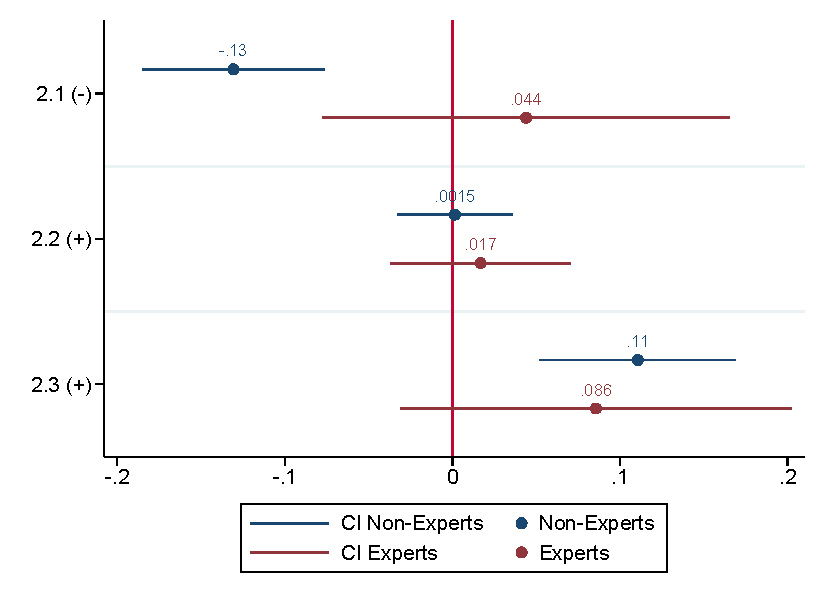
\includegraphics[scale=0.8]{Question2_base.pdf}
     \label{fig:my_label}
      \end{center}
      \tiny
     \tablenotes{The sign in parantheses denotes the predicted differential effect. Participants were asked to assess the following statements:  Question 2.1: The lender countries wanted to help the borrowing countries Question 2.2: The lender countries wanted to help themselves avoid a crisis at home Question 2.3: The lender countries wanted to impose institutional change upon the borrower countries  }
\end{figure}
 We continue to ask the participants about the emotions the rescue program evoked among citizens from the borrower and lender countries. The hypothesis that lenders have a blind spot regarding the feelings of citizens from borrower countries is confirmed. Participants from program countries in the non-expert sample are 9.2 and 9.3 percentage points more likely to agree that the rescue experience made them feel guilty and inferior. Further, the probability to agree to "The rescue experience made many citizens in the borrower countries feel exploited" increases by 16.9 percentage points among citizens from program countries. All effects are statistically significant at the 1 percent level. Among the sample of economic experts the effect sizes are smaller and not significantly different from zero. \\
 Interestingly, we do not find that borrowers have a blind spot regarding the emotions the program evoked among lender countries. There are only small differences in the likelihood to agree with certain statements between citizens from program and non-program countries which are not significant. There is no difference in evaluating the effect of the rescue program on the friendship between citizens. The results are similar in the expert and non-expert sample. \\

 We further predicted that borrower countries will be more confident that they will be able to repay outstanding debt. 
 When asked whether Greece \footnote{We only ask about Greece, since Greece remains the only country that has not repaid it's debt} will be capable of fully paying back it's debt, citizens from program countries show a 13.5 percentage point higher likelihood to agree in the non-expert sample and a 12.2 percentage point higher likelihood in the expert sample. This effect is again significant at the 1 percent level. \\
 \begin{figure} [h!]
    \begin{center}
    \caption{Hypothesis 4: Feelings evoked among citizens from program countries}
    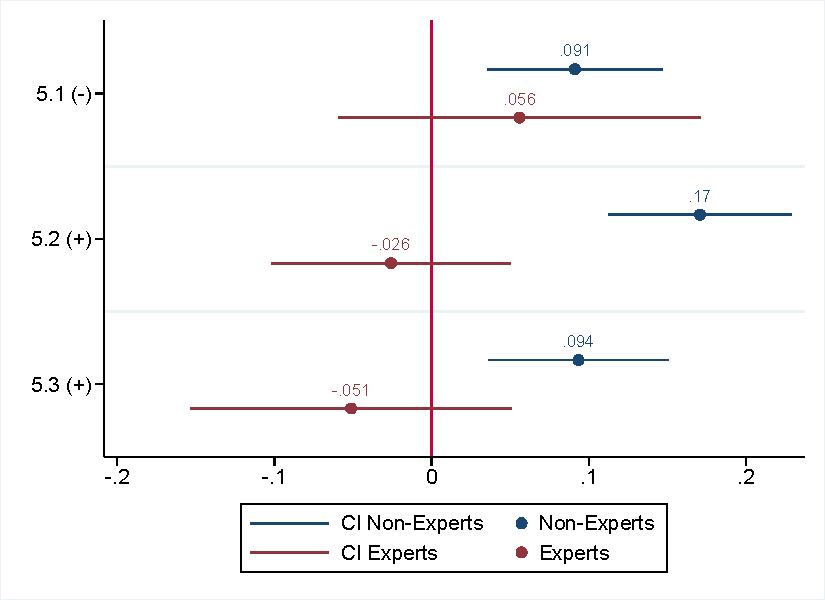
\includegraphics[scale=0.8]{Question5_1_base.pdf}
    \label{fig:my_label}
    \end{center}
    \tiny
    \tablenotes{The sign in parantheses denotes the predicted differential effect. Question 5.1: The rescue experience made many citizens in the borrower countries feel guilty; Question 5.2: The rescue experience made many citizens in the borrower countries feel exploited; Question 5.3: The rescue experience made many citizens in the borrower countries feel inferior. }
\end{figure}
\begin{figure}[h!]
\begin{center}
\caption{Hypothesis 4 and 5: Feelings evoked among citizens from non-program countries }

    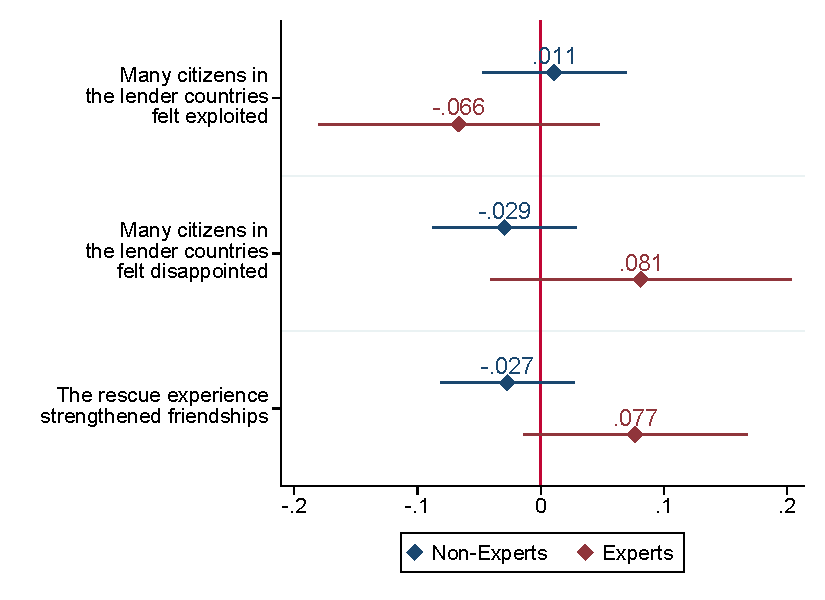
\includegraphics[scale=0.8]{Question5_2_base.pdf}
    \label{fig:my_label}
    \end{center}
    \tiny
    \tablenotes{The sign in parantheses denoted the predicted differential effect. Question 5.4: The rescue experience made many citizens in the lender countries feel exploited; Question 5.5 The rescue experience made many citizens in the lender countries feel disappointed Question 5.6: The rescue experience strengthened friendships between citizens Question 7: Greece will fully pay back it's debt}
\end{figure}
 
%  \begin{figure}
%\caption{Assessment of the emotions the program evoked among different parties}
%\centering
%\begin{minipage}{.5\textwidth}
% 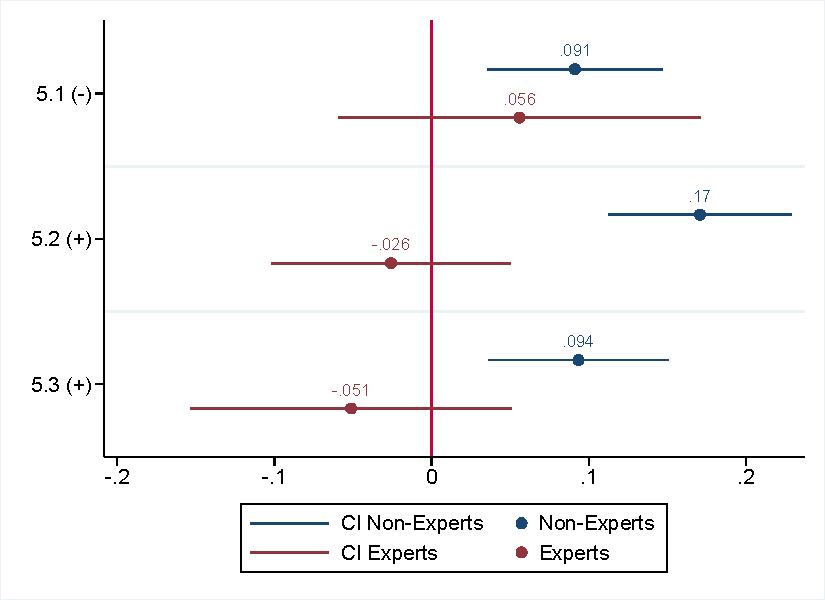
\includegraphics[scale=0.5]{Question5_1_base.pdf}
 %\end{minipage}%
 %\hfill
%\begin{minipage}{.5\textwidth}
%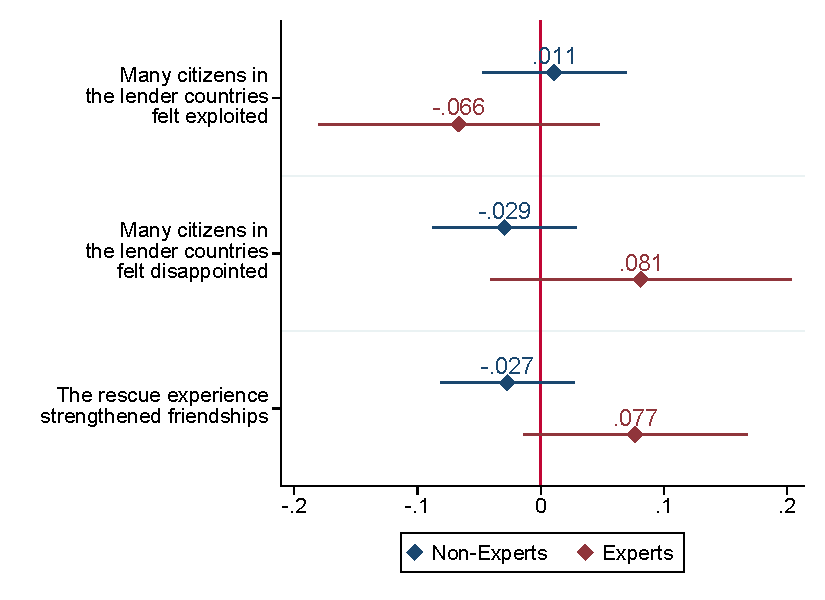
\includegraphics[scale=0.5]{Question5_2_base.pdf}
%\end{minipage}
%\end{figure}
 We proceed to evaluate who initiated and who benefited from the credit relationship. 
In the non-expert sample citizens are 13.2 percentage points more likely to state that the lender countries were the driving force behind signing the memorandum. Further, they are 28 percentage points more likely to state that the lender countries were the main beneficiaries of the program and 20.3 percentage points more likely to state that lender countries benefited from the loans to Greece. All effects are statistically significant at the one percent level. We do not find statistically significant effects in the expert sample. Interestingly, the mean difference between expert and non-experts is negative, contrary to the anticipated effect. Experts from program countries are for example 12.4 percentage points less likely to state that citizens from lender countries were the main beneficiary from the program.\\
\begin{figure}[h!] 
\begin{center}
     \caption{Hypothesis 2 and 3: Who initiated and benefited from the rescue program}
     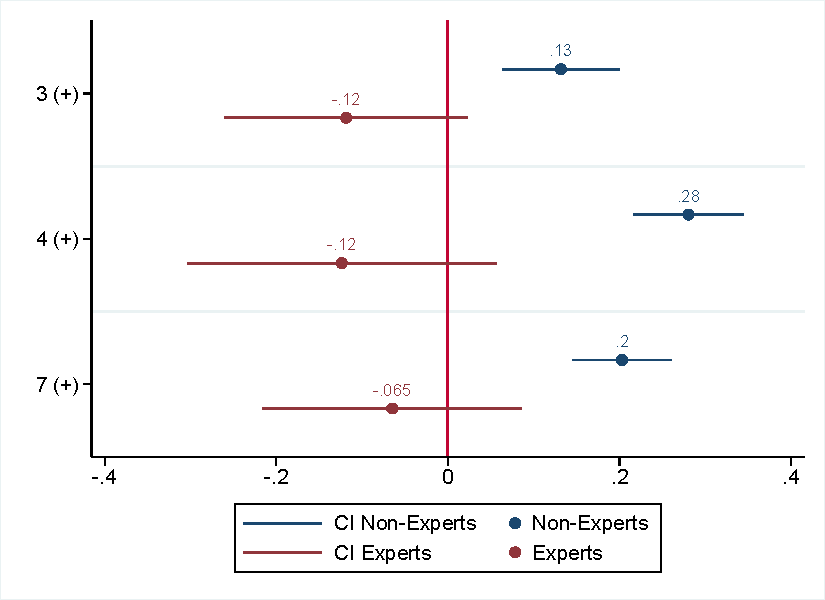
\includegraphics[scale=0.8]{Question3_base.pdf}
     \label{fig:my_label}
     \end{center}
     \tiny
     \tablenotes{The sign in parantheses denotes the predicted differential effect.Question 3: Who was the driving force behind signing the memorandum; Question 4: Who was the main beneficiary of the program; Question 7: Who primarily benefited from the loans to Greece}
\end{figure}

\textbf{Sample Splits}
Program and non-program countries vary along other dimensions than the program and non-program distinction. Program countries have some common characteristics that are likely to influence the estimates. Hence, we conduct sample splits along different macroeconomic variables to assess whether these macroeconomic characteristics influence the magnitude of our effect. Countries which were affected by the European debt crisis are predominantly Southern European and are located at the periphery of the European Union (measured by distance to Brussels). Further, all these countries experienced a substantial increase in debt levels, high levels of unemployment and low GDP growth. We also estimate our model on the subsample of all countries in the Eurozone. In the non-expert sample there are few changes to the baseline results, when splitting the sample along these different characteristics. When asked about the intentions behind entering the rescue program the findings from the baseline regression persist among all sample splits. The effect in the sample of countries with high levels of unemployment becomes smaller and is only significant at the five percent level. In the sample of southern European countries the disagreement over whether lender countries wanted to impose institutional change on borrower countries also decreases and is only significant at the five percent level. Interestingly, the estimates for the sample of periphery countries are much larger than in the baseline sample. In the periphery sample participants from program countries are 19.1 percentage points less likely to agree with the statement that the lender countries wanted to help the borrowing countries and 14.2 percentage points more likely to agree that lender countries wanted to impose institutional change compared to respectively 13.1 and 11.1 percentage points in the full sample.\\
When asked about the emotions of citizens in borrower and lender countries the estimates become slightly smaller in the southern European, periphery and high debt sample than for the full sample. The divergence in assessments about whether the rescue program made the citizens in the borrower countries feel inferior even becomes insignificant in the Southern European sample. Among all samples there is substantial disagreement between program and non-program countries that Greece will repay it's debt. 
\\
The magnitude and significance levels of effects of the program variable remains relatively unchanged for the remainder of questions. There are no differences in the effects of the full sample and all subsamples when asked about the driving force behind the referendum. Further, there is no difference in effects across samples when asked about the main beneficiary of the program. A detailed overview of the results across all sample splits is included in the appendix. 
\section{Heterogeneity Analysis and Robustness Checks}
Our results show that experts and non-experts show differences in their assessment of the European debt crisis. This finding is in line with work by \cite{roth} who using the WES and a representative sample show that experts differ from non-experts in their beliefs about the impacts of macroeconomic shocks. In our heterogeneity analysis we investigate which difference drives the observed results. We also examine whether individual factors influence the magnitude of the observed divergence. 
\\



\textbf{Socioeconomic Characteristics}
 Experts and non-experts differ along various dimensions such as education, age and gender.
 According to \cite{baumeister} events experienced at a younger age might have a more defining impact. Since the European debt crisis was accompanied for example by a high level of youth unemployment it might seem plausible that the divergences in memory might be more pronounced among the younger generation. Thus, we estimate the effect of belonging to a program country among participants older than 35 among the sample of non-experts.  The effect of the program variable on the likelihood to agree that the lender countries wanted to impose institutional change or that the rescue experience made citizens in the borrower countries feel guilty is smaller and the significance level decreases to 5 percent. For the remaining questions the overall magnitude and significance level of the program effect stays the same. 
\\
The level of education of participants may well influence the estimates. Participants with a higher level of education might have different political attitudes or consume and access different types of media. Hence, we split the non-expert sample and estimate our model only for participants reporting to have completed tertiary education. We do not find any change in the magnitude and significance level of effects for this subsample. 
\\
One dimension along which experts and non-experts differ is their degree of mobility. Experts working in think tanks or research institutes might live or have studied abroad for some time. Due to this circumstance experts might identify less with their nation than non-experts and consequently will not have a strong nation-serving bias. Unfortunately we don't have information about whether participants in the non-expert have lived or studied abroad. However, we can identify if people reported to be living in a different country than their country of birth. This applies to 25 percent of the non-expert subsample. 20.72 percent of participants from program countries and 25.45 percent from non-program countries report to be living in a different country than their country of birth. Estimating our model for this subsample changes the results quite a bit. Divergence between citizens from program- and non-program countries remains in the assessment if lender countries wanted to help borrowing countries and if the rescue experience made the citizens in the borrower countries feel exploited. For the other questions the difference in answers between program- and non-program countries becomes smaller and even vanishes completely for some questions. Hence, it appears that a higher level of mobility might be causal for the differential effects between expert and non-expert sample.  \\

\\
\textbf{Knowledge and beliefs} 
Participants differ in their level of knowledge about the European debt crisis. Some people fail to correctly identify their country as a borrower or lender country. An overview of the fraction of participants who knew their country's status can be found in the appendix. However, knowledge about the status of one's country does not appear to influence the observed effects. The estimates of the baseline model on the subsample of non-experts who could correctly identify their country does not change in comparison to the estimates for the full sample. 

\\\\
We redefine the program variable according to the beliefs of the survey participants. We now estimate the divergence in answers between participants which believed to be the national of a  lender country and participants which believed to be the national of a borrower country. Replacing the program variable by beliefs about belonging to a program country yields different results than the baseline model. In comparison to participants who believe to be lenders, participants who believe to be borrowers do not agree less that lender countries wanted to help borrower countries. They also do not agree more that the rescue program made citizens in the borrower countries feel guilty or inferior and or less likely to state that the lender countries were the driving force behind signing the referendum. Interestingly, differences emerge in the agreement about the feelings of citizens in the lender countries. Participants who believe they live in borrower countries are less likely to agree that citizens in the lender countries felt exploited or disappointed. They are further more likely to believe that the rescue program strengthened friendships between citizens. \\

\\
Our heterogeneity analysis yields some interesting observations about potential drivers of the observed differences between expert and non-expert sample. The comparison of means suggests that the observed differences are not driven by the opinion of experts resembling the opinion of non-experts from either program or non-program countries. 
Our analysis suggests that the observed difference between experts and non-experts cannot be explained by differential effects across age or education levels. However, it appears that non-experts which are more mobile do not show a strong nation-serving bias in their assessments of the European debt crisis. Interestingly, being able to correctly identify one's country as a program or a lender country does not change the observed magnitude of results. The magnitude of effects does change however, when redefining the program variable according to beliefs of people. This suggests that collective memory might work on a more subconscious level regardless of the level of information participants have. 
\\
\\
We also conduct various robustness checks. \\

\textbf{Ordered and Multinomial Estimation}
Participants have multiple answer possibilities. Depending on the question participants are able to rank their level of agreement on a scale of 1 to 4 or choose between the options borrower countries, lender countries or both equally. To control if differences between participants from non-program and program countries also emerge when including all answer possibilities as regression outcomes we estimate multinomial and ordered logit models. For all questions in which participants were asked to rank their level of agreement we estimate an ordered logit model, for questions in which participants were asked to name the responsible party we estimate an multinomial logit model. The significance level in the non-expert sample remains at the same level for all but one question. For the question which party was the driving force behind the referendum the significance level changes from 0.01 percent to 0.05 percent. In the expert sample all results remain insignificant. For the question if Greece will repay it's debt the divergence in effects is only significant at the 5 percent level and no longer the 1 percent level. In the majority of cases the the magnitude of effects is the same for different answer possibilities. This suggests that differences between program and non-program countries exist across all answer possibilities. \\

\\
\textbf{Inattentive Respondents}
Since we distributed our survey for the non-expert sample online we will also control for the influence of inattentive respondents in the non-expert sample. When distributing the survey online we already included an attention check when asking participants about socioeconomic characteristics. All participants failing this attention check were excluded from the survey. Further, we exclude all participants at the top 10 $\%$ and bottom 10 $\%$ of the survey time distribution. Excluding these participants does not change the inferences of our baseline estimation in the non-expert sample.\\


\\
\textbf{Clustered Robust Standard Errors} 
We cluster standard errors on the country level. Since we only collected data from 24 countries we adjust for the small number of clusters using the wild bootstrap method for logit regressions as suggested by \cite{cameron}.\footnote{We use the Stata command developed by \cite{roodman}} Inferences change for some questions when applying this method. Question 2.c becomes insignificant, questions 5a and 5c loose some significance and become significant at the 5 respectively 10 percent level.  \\

\textbf{Multiple Hypothesis Testing}
We also control for multiple hypothesis testing by adjusting our p-values using the Bonferroni Method. We adjust p-values by the number of questions we ask our participants. The Bonferroni correction does not change the significance level of our results. 


\section{Conclusion} 
The 2010 European public debt crisis influenced policies, politics and voters' perceptions. For example, domestic policy-makers introduced measures such as fiscal rules to handle increasing public debt and budget deficits. The European Central Bank pursued expansionary monetary policies: it introduced the Outright Monetary Transactions (OMT) program and decreased interest rates to zero. Rescue programs for Cyprus, Greece, Ireland, Portugal and Spain were designed. 

We examined citizens' views about the European public debt crisis. In particular, we investigated collective memory of the European public debt crisis and disentangled views of citizens from borrower countries and citizens from lender countries. During the public debt crisis, media reports have suggested that citizens from borrower and lender countries have different views on the crisis and how to handle it. Studies in psychology suggest that individual borrowers and lenders remember credit relationships in different manners (\cite{dezso}): memories are influenced by a self-serving bias. It is conceivable that such self-serving bias gives rise to a nation-serving bias in the memory of national credit relationships. We examine a nation-serving bias in memories of national credit relationships. Doing so is new.

We compiled new data measuring collective memories on the European debt crisis. We asked economic experts by using CESifo's World Economic Survey and non-experts by using the provider prolific. The results suggest that experts from lender and borrower countries have quite similar views about the European public debt crisis. The views of non-experts are, by contrast, influenced by a nation-serving bias. The bias relates to memories on why countries signed a memorandum and how they assess the measures taken to address the crisis. These results corroborate empirical studies about citizens' misperceptions about macroeconomic policies and outcomes. Citizens evaluate macroeconomic policies and outcomes much better when their preferred political party is in office than when parties govern that they do not support (on partisan bias see, for example, \cite{evans}, \cite{gerber}, \cite{gillitzer}, \cite{bachmann}). 

We observe a much smaller nations-serving bias among non-experts when we examine non-experts that left their country of birth. Cosmopolitans are less likely to evaluate European policies with a nation-serving bias than non-Cosmopolitans (see also \cite{bechtel}).

We believe that citizens' misperceptions and nation-serving bias in memorizing and handling European events are a major issue for European countries. When citizens have misperceptions and nation-serving bias in memorizing and handling European events, citizens are likely to demand policies that they would not demand when being suitably informed. Platforms of established political parties converged in many European countries. Established political parties did not wish to offer polarized in dealing with the public debt crisis. Many citizens were disenchanted and, in turn, new populist political parties entered the political arena. Clearly, citizens' views about the public debt crisis and their perceptions about European policies gave rise to electoral success of new (populist) parties and, in turn, reinforced policies in Europe. 

Our study shows divergences in how European policies between European countries are perceived. Moreover, experts who advise politicians do not tend to have misperceptions about the European public debt crisis. Misperceptions among non-experts but no misperceptions among experts and policy-makers may well explain why European policies and the EU as an institution is considered as unpopular in many countries. 

We believe that (social) media influence citizens' views a great deal. An avenue for future research is examining the extent to which social media influence misperceptions and nation-serving bias. 


\begin{table}[h!]

\caption{Which of the following statements do you agree with? (Regression Results 1 )} 
\hskip -2.5cm 
\begin{tabular}{l*{5}{c}}
\hline\hline
\ \  &Program & Clustered SE & Time Distribution & Bonferroni correction \\
\hline
\multicolumn{6}{l}{\textbf{2.a The Lender Countries wanted to help the borrowing countries}} \\
\ \   &-0.131{***}&-0.131{**}&-0.148{***} &-0.131{*** \\ 
&(0.028) & (0.028) & (0.031) & (0.028)  \\ 
\multicolumn{6}{l}{\textbf{2.b The Lender Countries wanted to help themselves to avoid a crisis at home}} \\
\ \  &0.001{}&0.001{}&0.005{}&0.001{} \\ 
&(0.018) & (0.018) & (0.019) & (0.018)   \\
\multicolumn{6}{l}{\textbf{2.c The Lender Countries wanted to impose institutional change upon the borrower countries }} \\
\ \   &0.111{***}&0.111{}&0.134{***} &0.111{***} \\ 
&(0.030) & (0.030) & (0.033) & (0.030) \\
\hline\hline
\end{tabular}
\begin{tablenotes}
\small
\item Standard-Errors in Parentheses \quad  ***p$<$0.01, **p$<$0.05, *p$<$0.1   
\end{tablenotes}
\end{table}
\begin{table}[h!]
\caption{Which of the following statements do you agree with? (Regression Results 1 )} 
\hskip -2.5cm 
\begin{tabular}{l*{5}{c}}
\hline\hline
\ \  &Program & Clustered SE & Time Distribution & Bonferroni correction \\
\hline
\multicolumn{5}{l}{\textbf{ 5a. The rescue experience made many citizens in the borrower countries feel guilty}} \\
\ \   &0.091{***}&0.091{**}&0.079{**} &0.091{**}\\ 
&(0.029) & (0.029) & (0.032) & (0.029)   \\ 
\multicolumn{5}{l}{\textbf{ 5b. The rescue experience made many citizens in the borrower countries feel exploited}} \\
\ \  &0.171{***}&0.171{***}&0.148{***}&0.171{***} \\ 
&(0.030) & (0.030) & (0.033) & (0.030)  \\
\multicolumn{5}{l}{\textbf{ 5c. The rescue experience made many citizens in the borrower countries feel inferior }} \\
\ \  &0.094{***}&0.094{*}&0.084{***}&0.094{**} \\ 
&(0.029) & (0.029) & (0.032) & (0.029)  \\
\multicolumn{5}{l}{\textbf{ 5d. The rescue experience made many citizens in the lender countries feel exploited}} \\
\ \   &0.011{}&0.011{}&-0.001{} &0.011{}\\ 
&(0.030) & (0.030) & (0.033) & (0.030)   \\ 
\multicolumn{5}{l}{\textbf{ 5e. The rescue experience made many citizens in the lender countries feel disappointed}} \\
\ \  &-0.030{}&-0.030{}&-0.033{}&-0.030{}\\ 
&(0.030) & (0.030) & (0.033) & (0.030)  \\
\multicolumn{5}{l}{\textbf{ 5f. The rescue strengthened friendships between citizens}} \\
\ \  &-0.025{}&-0.025{}&-0.040{}&-0.025{}\\ 
&(0.028) & (0.028) & (0.031) & (0.028) \\
\hline
\multicolumn{5}{l}{\textbf{7. Greece will fully pay back its debt}} \\
\ \   &0.133{***}&0.133{***}&0.129{***} &0.133{***}\\ 
&(0.022) & (0.022) & (0.024) & (0.022)   \\ 
\hline\hline
\end{tabular}
\begin{tablenotes}
\small
\item Standard-Errors in Parentheses \quad ***p$<$0.01, **p$<$0.05, *p$<$0.1  
\end{tablenotes}
\end{table}
\begin{table}[h!]
\caption{Which party was responsible for and benefitted most from the rescue package (Regression results 1) ?} 
\begin{tabular}{l*{5}{c}}
\hline\hline
\ \  &Program & Clustered SE & Time Distribution & Bonferroni correction \\
\multicolumn{5}{l}{\textbf{3. Who was the Driving Force behind signing the memorandum?}} \\
\ \  Lender Countries &0.132{***}&0.132{}&0.158{***} & 0.132{***} \\ 
&(0.035) & (0.035) & (0.038)& (0.035)\\ 
\multicolumn{5}{l}{\textbf{4. Who was the main beneficiary from the program? }} \\ 
\ \  Lender Countries &0.280{***}&0.280{}&0.282{***}& 0.280{***}\\ 
&(0.033) & (0.033) & (0.037) & (0.033)   \\
\hline
\multicolumn{5}{l}{\textbf{6. Who primarily benefited from the loans to Greece}} \\
\ \   &0.203{***}  &0.203{**}&0.205{***} &0.203{***}\\ 
   &(0.029) & (0.029) & (0.033) & (0.029)   \\ 
\hline\hline
\end{tabular}
\begin{tablenotes}
\small
\item Standard-Errors in Parentheses \quad  ***p$<$0.01, **p$<$0.05, *p$<$0.1   
\end{tablenotes}
\end{table}

\newpage
\bibliographystyle{plainnat}
\bibliography{bibliography.bib}
\end{document}
